\documentclass[12pt]{report}
\usepackage[utf8]{inputenc}
\usepackage[a4paper,width=150mm,top=25mm,bottom=25mm]{geometry}
\usepackage{amsmath}
\usepackage{amsfonts}
\usepackage{amsthm}
\usepackage{graphicx}
\usepackage{mathtools}

\setlength{\parskip}{1em}
% \setlength{\parindent}{0pt}

% \usepackage{setspace}
% document-wide settings:
%    \onehalfspacing

\usepackage{fancyhdr}
\pagestyle{fancy}

\newcommand{\thtitle}{The Even Subalgebras of Euclidean Geometric Spaces}
\newcommand{\thsubtitle}{The Realisation of Real Finite-Dimensional Associative Division Algebras in the Context of Euclidean Geometric Algebras}
\newcommand{\thauthor}{Marcelo Guimarães Neto}

\fancyhead[R]{\rightmark}
\fancyhead[L]{}

% \usepackage{biblatex}
\usepackage[style=alphabetic]{biblatex}
\addbibresource{res/references.bib}

\usepackage{lipsum}
\usepackage[dvipsnames]{xcolor}

\graphicspath{{res/images}}

% Available document structure commands:

% Book: \part{}, \chapter{}, \section{}, \subsection{}, \subsubsection{}, \paragraph{}, \subparagraph{}.

% Report: \part{}, \chapter{}, \section{}, \subsection{}, \subsubsection{}, \paragraph{}, \subparagraph{}.

% Article: \part{}, \section{}, \subsection{}, \subsubsection{}, \paragraph{}, \subparagraph{}.

% CUSTOM COMMAND DEFINITIONS
\newcommand{\R}{\mathbb{R}}
\newcommand{\C}{\mathbb{C}}
\newcommand{\HM}{\mathbb{H}}
\newcommand{\N}{\mathbb{N}}
\newcommand{\Z}{\mathbb{Z}}
\newcommand{\Q}{\mathbb{Q}}
\newcommand{\E}{\mathbb{E}}
\newcommand{\G}{\mathcal{G}}
\newcommand{\V}{\mathcal{V}}

\newcommand{\mg}[1]{\left|#1\right|}
\newcommand{\bv}[1]{\boldsymbol{#1}}
\newcommand{\gs}[1]{\langle #1 \rangle}
\newcommand{\g}[2]{\langle #1 \rangle_{#2}}
\newcommand{\gr}[1]{\mathrm{gr}\left(#1\right)}

% THEOREM ENVIRONMENT DEFINITIONS
\newtheorem{theorem}{Theorem}[section]

\theoremstyle{definition}
\newtheorem{definition}{Definition}[section]

\theoremstyle{definition}
\newtheorem{axiom}[definition]{Axiom}

\newtheorem{lemma}[theorem]{Lemma}
\newtheorem{corollary}[theorem]{Corollary}
\newtheorem{example}[definition]{Example}

\theoremstyle{remark}
\newtheorem*{remark}{Remark}


%%%%%%%%%%%%%%%%%%%%%%%%%%%%%%%%%%%%%%%%

\begin{document}

\begin{titlepage}
    \begin{center}
        % \vspace*{1cm}
            
        \Huge
        \textbf{\thtitle}
            
        \vspace{0.5cm}
        \LARGE
        \thsubtitle  
        
		\vspace{1cm}
        \Large    
        Author: \textbf{Marcelo Guimarães Neto}
		
		Supervisor: \textbf{Konstantin Izyurov}

        \vfill
        A thesis presented for the degree of\\
        Bachelor of Science
            
        \vspace{0.8cm}
        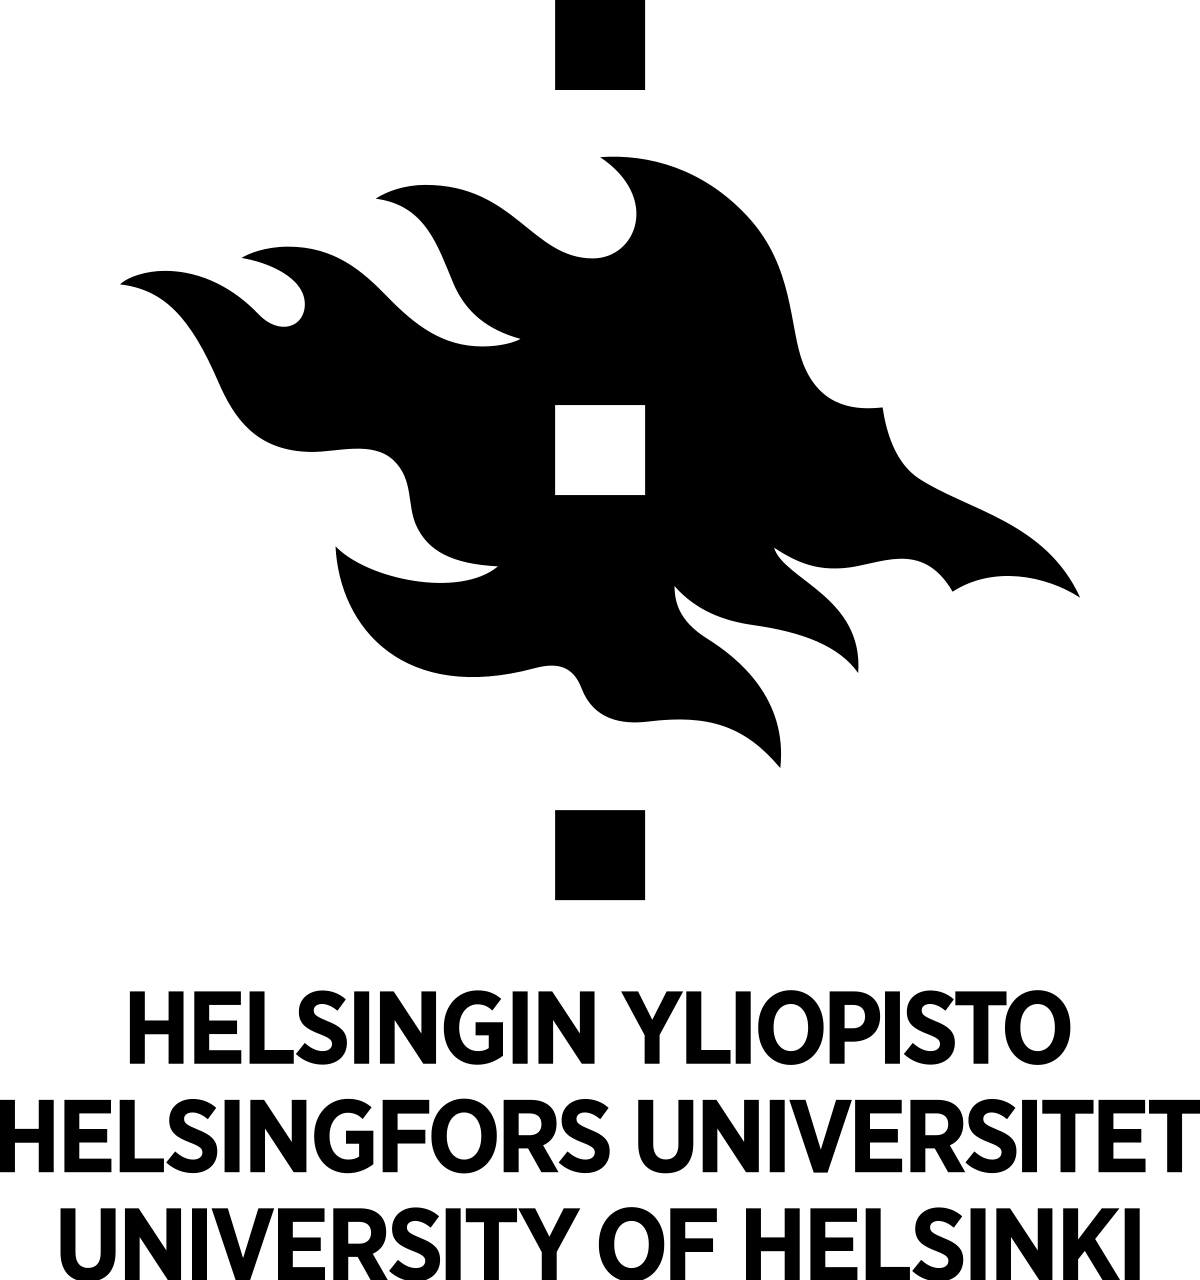
\includegraphics[width=0.4\textwidth]{heluni-logo.png}
        
        \vspace{0.8cm}
        Department of Mathematics and Statistics\\
        Faculty of Science\\
        University of Helsinki\\
        Finland\\
        \today
            
    \end{center}
\end{titlepage}


\thispagestyle{plain}
\begin{center}
    \Large
    \textbf{The Even Subalgebras of Euclidean Geometric Spaces}
        
    \vspace{0.4cm}
    \large
    A Geometric Proof of the Frobenius Classification of Finite-Dimensional Associative Division Algebras over the Reals       

    \vspace{0.4cm}
    \textbf{Marcelo Guimarães Neto}
       
    \vspace{0.9cm}
    \textbf{Abstract}
\end{center}
Lorem ipsum dolor...


\chapter*{Acknowledgements}
I want to thank...

\tableofcontents
\listoftables

\chapter{Introduction}
\section{Historical Background}
Geometric Algebra has its roots in the long-running pursuit of a mathematical framework for the description of physical space. Though the concept of vectors is ancient, in this section we shall focus on the developments starting in the 19th century.

In the early 1800s, \textbf{Grassmann} was the first to formulate the notions of 'modern' linear algebra (vector spaces, bases, inner product and orthogonality); his development of exterior algebra through the introduction of the outer product, laid the key theoretical groundwork for Clifford's Geometric Algebra as it provided a formal algebraic system for vectors which is capable of describing higher-dimensional geometric primitives (p.28-29)\cite{ga-foundations}:
\begin{align*}
	\bv{e_i} | \bv{e_j} &= \delta_{ij}\\
	\bv{e_i}\wedge \bv{e_j} &= -\bv{e_i}\wedge \bv{e_j}\\
\end{align*}

Around the same time, \textbf{Hamilton} extends the 2-dimensional algebra of the complex numbers into the 4-dimensional algebra of the quaternions, aiming at a formal vector algebra for $\mathbb{R}^3$.
\begin{align*}
    &q = q_0 + q_1\boldsymbol{i} + q_2\boldsymbol{j} + q_3\boldsymbol{k}\\
    &i^2 = j^2 = k^2 = ijk = -1\\
    &ij = k, ki = j, jk = i
\end{align*}

The quaternion algebra, though arithmetically complete and initially adopted by Maxwell in his formulation of electrodynamics, was not very popular due to its noncommutativity and the negative square of vectors, and eventually became relegated to very specific applications. Fundamentally, the shortcomings of the quaternions are grounded in the fact that quaternions provide a representation for the algebra of rotations in three-dimensions, and are not suitable to describing cartesian vectors in $\R^3$ \cite{ga-history}.

\textbf{Gibbs} is responsible for the standard vector algebra that is most widely used today: his insight was to separate the product of quaternion 'vectors' into dot and cross products and formally replace the imaginary units with unit vectors that square to $+1$.
\begin{align*}
	vu &= -\sum v_iu_i + \sum_{i\to j\to k}(v_iu_j - v_ju_i)\boldsymbol{k} \\
	&\equiv -v | u + v \times u
\end{align*}

The development of standard vector calculus (e.g. $\nabla, \nabla \cdot, \nabla \times$), applied extensively in Electrodynamics by \textbf{Heaviside}, lead to the widespread adoption of the formalism.

Though it became the adopted formalism, \textbf{Gibbs}' vector algebra has its own deficiencies: it requires two different vectors product, lacks a division operation, the cross product is noncommutative and does not generalize to higher-dimensions.

\textbf{Clifford}'s  Geometric Algebra - introduced in the second half of the 19th century - aimed to supersed both formalisms by providing an arithmetically complete algebra that could be generalized to higher dimensions, and adequately describe both vectors and transformations in space; it extends Grassmann's work, incorporating Hamilton's quaternions into an abstractable and generalizable algebraic system for vectors, based on the geometric product:
\begin{align*}
    &uv = u | v + u \wedge v\\
    &V = \sum \langle V\rangle_i\\
    &\g{V}{r} = \sum v_i\bv{e_{i_1}}\wedge ... \wedge \bv{e_{i_r}}
\end{align*}

Though \textbf{Clifford}'s work was neglected in his time, it has recently been repopularized by \textbf{David Hestenes} \cite{ga-origin}. We will be discussing the modern formalism in this thesis.

\newpage

\section{Content and Aim}

Geometric Algebra - as the mathematical project proposed by \textit{David Hestenes} and \textit{Garret Sobczyk} in \cite{ga-origin} - is a relatively new subject: as such, there seems to be no consolidated consensus as to the precise manner in which it ought to be presented. This paper will follow most closely the original approach in \cite{ga-origin}; nonetheless, I have taken the liberty to formulate and present some of these concepts in a slightly different manner (though only superficially so). In particular, this applies to the choice of axioms - inspired by \textit{Eric Chisolm}'s take on the topic \cite{ga-chisolm} - and the formulation of the \textbf{Universal Geometric Algebra} as a family of abstract algebras.

\textbf{Geometric Algebra} concerns itself with the construction of a collection of abstract algebras which adequately extend the arithmetic of the real numbers to higher-dimensional, coordinate-free settings, under the guidance of geometric intuition. In a \textbf{Geometric Algebra} elements are fully characterised by three (geometric) properties: \textbf{magnitude}, \textbf{direction} and \textbf{orientation}. In practice, the theory identifies linear spaces with Euclidean geometric primitives, and in doing so equips any (finite-dimensional) linear space with a powerful algebra whose elements are the subspaces themselves.

This is reminiscent of the Greek pre-algebraic view of mathematics, whereby arithmetic was intrinsically tied to geometric constructions. 
Perhaps for this very reason, \textbf{Geometric Algebra} has had made significant progress in its express goal of providing a unified framework for mathematical physics and applied mathematics. In his book, \textit{Hestenes} details this more specifically (p. ix)\cite{ga-origin}:

\begin{quote}
	``Our long-range aim is to see Geometric Calculus established as a unified system for handling linear and multilinear algebra, multivariable calculus, complex variable theory, differential geometry and other subjects with geometric content.''
\end{quote}

Our main focus in this paper, will be in the mathematical exposition of the theory: we will be proving basic properties and theorems from the axioms and use these towards constructing the Euclidean Geometric Algebras and their Even Subalgebras in 1, 2 and 3 dimensions, demonstrating that the latter are actually isomorphic to the Real, Complex and Quaternion algebras.


\chapter{Mathematical Background}
\section{Abstract Algebra: A Brief Primer}

\subsection{Groups, Rings and Fields}
\begin{definition}[Group]
    A group is a set closed under an associative, invertible product.
\end{definition}   

\lipsum[1-3]

\begin{definition}[Ring]
    A ring is an Abelian group (we refer to the group operation as addition) equipped with a second associative and distributive binary operation (we refer to it as multiplication).
\end{definition}


\lipsum[1-5]

\begin{definition}[Field]
    A field is a commutative ring in which every non-zero element has a multiplicative inverse.
\end{definition}


\lipsum[3-5]

\subsection{Modules, Vector Spaces and Algebras}
\lipsum[1-2]

\begin{definition}[Module]
    A module is an Abelian group closed under a left-right multiplication by a ring that is associative and distributive.
\end{definition}

\lipsum[1-5]

\begin{definition}[Vector space]
    A vector space is a module over a field.
\end{definition}

\lipsum[1-2]

\begin{definition}[Algebra]\label{d:algebra}
    A real algebra $A$ is a real vector space equipped with a bilinear product; i.e. a set equipped with two operations ($+, \cdot: A\times A \to A$) and an action ($*: \R \times A \to A$) under which it is closed, having the following properties:

	\begin{itemize}
		\item The addition operation is associative, invertible and commutative.
		\item The action (or multiplication by scalar) is associative and distributive with regards to the addition operation.
		\item The product (or multiplication) is bilinear:
				\[(a*x + y)\cdot (b*z + t) = ab*xz + a*xt + b*yz + yt\]
	\end{itemize}

%    \[\begin{alignedat}{3}
%        &+ &&: \ &&\text{associative, invertible, commutative}\\
%        &\cdot &&: \ &&\text{bilinear}: (a*x + y)\cdot (b*z + t) = \\
%        & && &&= ab*xz + a*xt + b*yz + yt  \\
%        &* &&: \ &&\text{associative, distributive}
%    \end{alignedat}\]

\end{definition}

\lipsum[1-3]

\begin{definition}[Homomorphisms]
	An algebra \textbf{homomorphism} is a map between two algebras which preserves their algebraic structure, i.e. $\varphi: A \to B$ s. that $\forall a \in \R$ and $x, y, z \in A$:
    \[\varphi(a*xz+y) = a*\varphi(x)\varphi(z) + \varphi(y)\]
	If the mapping is 1-to-1, we call it an \textbf{isomorphism}.
\end{definition}

\lipsum[1-2]

DIVISIBILITY
\lipsum[1-3]

\begin{definition}[Division Algebra]\label{d:division-algebra}
	An associative algebra $A$ is a \textbf{division algebra} iff all non-zero elements have a multiplicative inverse, i.e.
	\[\forall a \in A \ \exists x \in A \ \mathrm{s. that} \ ax = xa = 1\]
\end{definition}

\lipsum[1-5]


\chapter{Geometric Algebra}
\section{The Universal Geometric Algebra}\label{s:uga}

In the standard formalism, the fundamental concept in Geometric Algebra is that of the \textbf{Universal Geometric Algebra} (UGA for short): an infinite-dimensional abstract algebra obeying a certain set of axioms, within which all the Geometric Algebras are contained (as subalgebras) \cite{ga-origin}. 

For our purposes, whereby we will limit ourselves to geometric algebras over finite-dimensional inner product spaces, I have found this to be unnecessary and not the best suited approach. Instead we shall formulate as our starting point, a family of geometric algebras:
\begin{definition}[Geometric Family of Algebras]
	The \textbf{Geometric Family of Algebras} is a family of algebras obeying a specific set of axioms. Its elements (the Geometric Algebras) are specified by the choice of a finite-dimensional inner product space over the real numbers.
\end{definition}

A \textbf{GFA} is then a template for Geometric Algebras: given a finite-dimensional linear space, and an inner product, there exists a unique axiom-abiding algebra which contains the linear space and whose symmetrized product corresponds to the prescribed inner product.

We will, however, discuss the generally applicable definitions and results in the context of an abstract algebra whose formal product obeys the axioms, and whose abstract linear space will always be assumed to be of a sufficiently high (finite) dimension such that it does not get in the way of the argument.

\newpage

\section{Axioms and Definitions}\label{s:axioms-definitions}

The Geometric Algebra $\G$ of a finite-dimensional inner product space $\V$ is the 'freest' (i.e. the most general) unitary associative algebra over the reals obeying the following axioms:
\begin{axiom}\label{a:ga-axiom1}
    $\G$ contains $\R$ as a subalgebra and $\V$ as a subspace; these generate the entire algebra. We call elements of $\R$ scalars, and elements of $\V$ vectors.
\end{axiom}

\begin{axiom}\label{a:ga-axiom2}
	The formal product of a scalar and a vector corresponds with the multiplication by a scalar of the vector space.
\end{axiom}

\begin{axiom}\label{a:ga-axiom3}
    The square of a vector corresponds to its inner product with itself.
	\[\forall v \neq 0 \in \V \quad v^2 \equiv vv = v|v = |v|^2\]
\end{axiom}

%\begin{axiom}\label{a:ga-axiom4}
%	The formal product on $\V$ is positive-definite, i.e.:
%\[\forall v \neq 0 \in \V \quad vv > 0\]
%\end{axiom}

\begin{remark}\label{r:ga-axiom3}
	The above axiom distinguishes a Clifford Algebra from a Geometric Algebra in our treatment: a Clifford Algebra only requires a quadratic form on a vector space $\V$. Standard treatments of Geometric Algebra also do not make such a strict requirement and thus the terms are often used interchangeably: we will not be doing so in this thesis.
\end{remark}

%\begin{axiom}\label{a:ga-axiom5}
%%	The antisymmetrized product of linearly independent vectors	produces an element which does not belong to $\R \bigoplus \V$, we call this product the \textbf{exterior product} and denote it $u \wedge v = \frac{1}{2} (uv - vu)$. 
%	The product of linearly independent vectors produces an element that is not in the linear span of its factors: i.e. if $\{v_i\}_{i=1}^n$ is a linearly independent set, then:
%	\[\prod_{i=1}^n v_i \notin \mathrm{span}\{\prod_{j=1}^n v_{i_j} \forall i_j : \{1..n\} \to \{0..n\} \} \equiv F(\{v_i\}_{i=1}^n)\]
%	were we define $v_0 = 1$ for notational convenience.
%\end{axiom}

We refer to the product of such an algebra as a \textbf{geometric product}.

\begin{remark}
	That the algebra is the 'freest' simply means that we specify the product just enough that it satisfies the axioms, and impose no further relations. One could for example define a geometric product on $\R^3$ as the sum of the inner and cross products: the generated algebra would satisfy the axioms, however it would not be the freest since the cross product imposes the additional equivalence relation:
	\[e_ie_{[i+1]_3} \equiv e_{[i+2]_3} \quad \forall i \in \{1,2,3\}\]
	where $[a]_3$ is a shorthand notation for $a$ mod $3$.
	A modern, abstract formulation of the concept has this property naturally since the Geometric Algebra is constructed from more abstract objects by imposing only the required relations: I have not taken this route given the scope and target audience of the thesis. \textcolor{red}{FETCH A REFERENCE?!}
\end{remark}

Two results follow immediately from Axiom \ref{a:ga-axiom3}:
\begin{lemma}\label{l:invertibility}
	All vectors are invertible with respect to the geometric product and the inverse is given by:
	\[v^{-1} = \frac{v}{\mg{v}^2}\]
\end{lemma}



\begin{lemma}[Inner Product]\label{l:inner-product}
	The symmetrized product of two vectors, \[s(u,v) = \frac{1}{2}(uv + vu)\] corresponds to the inner product on $\V$, i.e.: \[s(u,v) = u|v \forall u,v \in \V\]
\end{lemma}

\begin{proof}
	Consider the following expression, and recall Axiom \ref{a:ga-axiom3}:
    \begin{align*}
        &(u+v)^2 = u^2 + v^2 + uv + vu \Leftrightarrow \\
        &2u|v = (u+v)^2 - u^2 - v^2 \in \R
    \end{align*}
	So the symmetrized product maps into $\R$ (i.e. $| : \V \times \V \to \R$). By Definition \ref{d:algebra}, the geometric product is bilinear and so is the symmetrized product as it is a linear function of the bilinear products; moreover, by Axiom \ref{a:ga-axiom4}, it is also positive-definite. We conclude that $u|v = uv + vu$ is indeed an inner product on $\V$.
	
\end{proof}


%We have seen that $\R \bigoplus \V$ is closed under the symmetric part of the product; the algebra must thus be generated by the antisymmetric part of the product:
%\begin{definition}[Exterior Product]\label{d:exterior-product}
	The linear rejection $R(\prod_{i=1}^n, F(\{v_i\}_{i=1}^n))$ of a product with regards to the linear span of its factors is denoted
	\[ \bigwedge_{i=1}^n v_i \equiv v_1 \wedge ... \wedge v_n \]
	We call this exterior (or outer) product.
\end{definition}


We have observed that the axioms place a restriction on the symmetric part of the product between two vectors. The antisymmetric part, on the other hand, bears no restriction: since the Geometric Algebra is the most general algebra obeying the axioms, we identify this part of the product with a formal bilinear and antisymmetric product, we call it the \textbf{exterior} product. We thus obtain the principal property of the geometric product.
\begin{theorem}[Geometric Product of Vectors]
	The geometric product of two vectors can be broken down into an inner and an exterior product: \[uv = u | v + u \wedge v\]
\end{theorem}

\begin{proof}
	We first show how the geometric product decomposes into a symmetric and antisymmetric part:
	\[uv = \frac{1}{2}(uv + uv) = \frac{1}{2}(uv + vu + uv - vu) = \frac{1}{2}(uv + vu) + \frac{1}{2}(uv - vu)\]
	The result follows immediately from Lemma \ref{l:inner-product} and Axiom \ref{a:ga-axiom5}:
	\[uv = u | v + u \wedge v\]
\end{proof}


As a corollary, we obtain the following self-evident propositions.
%\begin{corollary}
	The exterior product of a linearly dependent set of vectors is zero.
\end{corollary}

%\begin{proof}
	PROBLEM: exterior product is currently defined in terms of geometric product only for two vectors...
	Let $\{v_i\}_{i=1}^n$ be a linearly dependent set of vectors, i.e.:
	\[\exists \{\alpha_i\}_{i=1}^{n-1} : v_n \equiv \sum_{i=1}^{n-1} \alpha_i v_i\]
	Then, consider their outer product and recall bilinearity and antisymmetry:
	\begin{align*}
		\bigwedge_{i=1}^n v_i &= v_1 \wedge ... \wedge \sum{i=1}^{n-1} \alpha_i v_i \\
		&= (\bigwedge_{i=1}^{n-1} v_i) \
\end{proof}

\begin{corollary}
	A pair of vectors are orthogonal if and only if they anticommute with respect to the geometric product.
\end{corollary}


\begin{corollary}\label{c:orthonormal-bases}
	An orthonormal basis $\{e_i\}_{i=1}^n$ obeys the following relations:
	\begin{align*}
		e_ie_j &= -e_je_i \\
		e_ie_i &= 1
	\end{align*}
\end{corollary}


Before we make some final remarks about existence, uniqueness and construction, we ought to familiarise ourselves with some specific terminology.
\begin{definition}
	We refer to reals $a \in \R \subset \G(\V)$ as \textbf{scalars}, or $\textit{grade-0}$ vectors.
\end{definition}
\begin{definition}
	Elements $v \in \V \subset \G(\V)$ are called \textbf{$1$-vectors}, or simply vectors.
\end{definition}
\begin{definition} \label{d:k-blades}
	A \textbf{$k$-blade} is a product $e_{i_1}e_{i_2} \ldots e_{i_k}$ of orthogonal vectors; these are also called simple $k$-vectors.
\end{definition}
\begin{definition}
	A \textbf{versor} is an arbitrary product $v_1v_2 \ldots v_k$ of vectors.
\end{definition}
\begin{definition}
	\textbf{Multivectors} are finite sums of versors. By Axiom \ref{a:generation}, every element $V \in \G(\V)$ is a multivector.
\end{definition}


A critical lemma to which we will often make implicit reference is the following:
\begin{lemma}\label{l:ga-expansion}
	Every element $V \in \G(\V)$ has a unique decomposition (with respect to a given basis) as a sum of k-blades.
\end{lemma}

\begin{proof}
	Every multivector can be written as a finite sum of versors, so it suffices to prove the statement for an arbitrary versor.
	Consider an arbitrary set of vectors expressed in a given orthonormal basis $\{v_i \equiv \sum_{j=1}^n v_i^je_j\}_{i=1}^m$; we expand their product using bilinearity:
	\[\prod_{i=1}^m v_i = \prod_{i=1}^m \sum_{j=1}^n v_i^j e_j = \sum_{j_i : \{1..m\} \to \{1..n\}} \left(\prod_{i=1}^m v_i^{j_i}\right) \left(\prod_{i=1}^m e_{j_i}\right)\]
	It follows from Corollary \ref{c:orthonormal-bases} that the product of the basis vectors in each term is a $k$-blade, where $k$ is the number of unit vectors appearing an odd number of times in the product.
	Uniqueness follows from the freeness of the algebra: the product of orthogonal vectors is a formal product subject only to bilinearity and antisymmetry, so that distinct products of orthonormal basis vectors are linearly independent and form in fact a vector space-basis for the whole algebra.
\end{proof}


We are now justified in presenting the following definitions:
\begin{definition}[Grade]\label{d:grade}
	We introduce the grade operator $\g{A}{k}$ which returns the $k$-grade component of $A$.
	The grade of a multivector $\gr{A} \in \N$ is the grade of the maximum-grade term in $A$.
	We say $A$ is a \textbf{homogeneous} multivector of grade $k$ iff it is a sum of $k$-blades for a given $k \in \N$ (when we wish to make it explicit, we denote it $A_k$); otherwise we say $A$ is of mixed grade.
\end{definition}

\begin{definition}[Basis]\label{d:basis}
	The \textbf{basis} of a Geometric Algebra $\G(\V)$ is simply the basis of the generating inner-product space $\V$.
\end{definition}

\begin{definition}
	A \textbf{frame} of a Geometric Algebra $\G(\V)$ is the set of distinct (up to permutation) $k$-blades formed from an orthogonal basis of $\G(\V)$.
\end{definition}

\begin{definition}
	The \textbf{pseudoscalar} of a geometric algebra $\G(\V)$ is the highest grade element in its frame. It is unique up to scalar multiplication and including permutation of factors.
	The square of a pseudoscalar is a scalar: by convention, it is normalized such that it squares to $1$ or $-1$ (defining the orientation of the frame).
\end{definition}


The distinction between basis and frame is very important: a frame is to a basis, as a geometric algebra is to its generating vector space.
For finite-dimensional spaces, we can always produce an orthonormal basis by the Gram-Schmidt process, so we will henceforth assume all bases to be orthonormal unless otherwise specified.

A frame can be identified one-to-one with the power set of a basis, as it is composed of all the possible combinations of the basis elements without repetition and up to permutation (we identify the unit scalar in the frame with the empty subset of the basis). It follows that the dimension of a geometric algebra $\G$ (as a vector space) is $2^{\gr{\G}}$.

It is then clear that for every inner product space there exists a unique Geometric Algebra, and the recipe for its construction is quite simple:
\begin{enumerate}
	\item construct an orthonormal basis for the inner-product space: this will be the basis of the algebra
	\item construct the frame of the algebra by taking products of basis vectors
	\item generate the rest of the algebra as a vector space with the frame as its basis
\end{enumerate}

% With the above terminology we can also straightforwardly prove the Universal Property of a Geometric Algebra.
% \begin{definition}[Universal Property of a Geometric Algebra]
	Let $\V$ be a finite-dimensional vector space over the reals, and let $j: \V \times \V \to \R$ be an inner product, then there exists unique geometric algebra $\G(\V)$ and canonical injection $i: \V \to \G(\V)$ such that the following diagram commutes:
	\textcolor{red}{NOT QUITE!}
\end{definition}

% \begin{definition}[Universal Property of a Geometric Algebra]
	Let $\V$ be a finite-dimensional vector space over the reals, and let $j: \V \times \V \to \R$ be an inner product, then there exists unique geometric algebra $\G(\V)$ and canonical injection $i: \V \to \G(\V)$ such that the following diagram commutes:
	\textcolor{red}{NOT QUITE!}
\end{definition}


A brief note on conventions: here on out, whenever left unspecified, the precedence of products is inner$\to$wedge$\to$geometric.

%\newpage
%
%\section{Construction: Bases and Frames}\label{s:bases-frames}
%
%A Geometric Algebra is only realized into a concrete algebra once an inner-product space is specified. It is then straightforward to construct the whole algebra given a basis for the inner-product space. But first, we need some specific terminology.


\newpage

\section{Products}\label{s:products}
We will now go on to consider general expressions and properties of products between arbitrary multivectors.
First off, we generalize the definition of the inner and outer products to homogeneous multivectors.
\begin{definition}\label{d:inner-product1}
	The inner product $A_r|B_s$ between two homogeneous multivectors $A_r$ and $B_s$ is the lowest-possible grade term in their product. We will later see that this is the $\mg{r-s}$-grade term; if the product does not have such a term, then we say that the inner product is 0.
\end{definition}

\begin{definition}\label{d:outer-product1}
	The outer product $A_r \wedge B_s$ between two homogeneous multivectors $A_r$ and $B_s$ is the highest-possible grade term in their product. We will later see that this is the $\mg{r+s}$-grade term; if the product does not have such a term, then we say that the outer product is 0.
\end{definition}


We now prove the following lemma regarding the product of a vector with a homogenous multivector.
\begin{lemma}\label{l:v-mv-product}
	The inner and outer products of a vector with a homogeneous multivector have the following expressions:
	\begin{align*}
		& a | A_r = \g{aA_r}{r-1} = \frac{1}{2}(aA_r-(-1)^rA_ra) \\
		& a \wedge A_r = \g{aA_r}{r+1} = \frac{1}{2}(aA_r+(-1)^rA_ra)
	\end{align*}
\end{lemma}

\begin{proof}
	We shall assume that $A_r$ is an $r$-blade: the case of a homogeneous multivector follows directly using distributivity of the geometric product (since an $r$-grade homogeneous multivector is a sum of $r$-blades).

	Recall the definition of the inner product between two vectors (def. \ref{d:inner-product1})
	\[a | b = \frac{1}{2}(ab + ba)\]
	We can reverse it to obtain:
	\[ab = 2 a | b - ba\]
	Repeated application of the above allows us to permute indices in a product, as follows:
	\begin{align*}
		aA_r = aa_1a_2 \ldots a_r = &2a|a_1a_2 \ldots a_r - a_1aa_2 \ldots a_r \\
		= &2a|a_1a_2 \ldots a_r - 2a|a_2a_1 \ldots a_r + a_1aa_2 \ldots a_r \\
		= &\ldots \\
		= &2 \sum_{k=1}^r (-1)^{k+1}a|a_k a_1 \ldots \check{a_k} \ldots a_r + (-1)^ra_1a_2 \ldots a_ra \\
		= &\sum_{k=1}^r (-1)^{k+1}a|a_k a_1 \ldots \check{a_k} \ldots a_r + \sum_{k=1}^r (-1)^{k+1}a|a_k a_1 \ldots \check{a_k} \ldots a_r \\
		&+ (-1)^ra_1a_2 \ldots a_ra
	\end{align*}

	Notice that the first term above has grade $r-1$: we will demonstrate that this is indeed the lowest grade term. For now, we preemptively denote it $a | A_r$.
	
	Let us rewrite the sum using invertibility of vectors (th. \ref{l:invertibility}):
	\begin{align*}
		a | A_r &= \sum_{k=1}^r (-1)^{k+1}a|a_k a_1 \ldots \check{a_k} \ldots a_r\\
				&= \sum_{k=1}^r (-1)^{k+1}a|a_k a_k^{-1}a_k a_1 \ldots \check{a_k} \ldots a_r\\
				&= \sum_{k=1}^r a|a_k a_k^{-1} A_r 
	\end{align*}

	Substracting the above from $aA_r$ and factoring:
	\[aA_r - a | A_r = (a - \sum_{k=1}^r a|a_k a_k^{-1})A_r \equiv bA_r\]
	
	Since by construction, $b | a_k = 0 \forall k \in \{1, \ldots r\}$, it follows by Corollary \ref{c:orthogonality} that the above is a product of $r+1$ anticommuting vectors and thus has grade $r+1$ by Definition \ref{d:k-blades}. We are justified in writing:

	\begin{align*}
		aA_r &= a | A_r + a \wedge A_r \\
		a | A_r &= \sum_{k=1}^r (-1)^{k+1}a|a_k a_1 \ldots \check{a_k} \ldots a_r \\
		a \wedge A_r &= a | A_r + (-1)^rA_ra
	\end{align*}

	From which the lemma follows straightforwardly by substituting the third expression into the first:
	\begin{align*}
		aA_r &= 2a | A_r + (-1)^rA_ra \Rightarrow a | A_r = \frac{1}{2} (aA_r - (-1)^rA_ra) \\
		aA_r &= 2a \wedge A_r - (-1)^rA_ra \Rightarrow a \wedge A_r = \frac{1}{2} (aA_r + (-1)^rA_ra)
	\end{align*}
\end{proof}


The above proof is due to \textit{Hestenes} (p. 8-10)\cite{ga-origin}

Using the above lemma, we can prove the following important property of the geometric product between homogeneous multivectors.
\begin{theorem}[Product of Homogeneous Multivectors]\label{t:homog-product}
	The product of homogeneous multivectors $A_r, B_s$ can be decomposed as follows:
	\[A_rB_s = \sum_{k=0}^{\min\{r,s\}} \g{A_rB_s}{\mg{s-r}+2k}\]
\end{theorem}

\begin{proof}
	We prove this by induction on $r \leq s$ when $A_r$ and $B_s$ are simple $r$- and $s$-vectors respectively.

	The case $r=1,\ s=1$ is true by Definition \ref{t:geometric-product}.
	The case $r=1,\ s>1$ is true by Lemma \ref{l:v-mv-product}.
	Assume the expression holds for $r = q,\ s > r$, we show that it holds for $r+1$:
	\begin{alignat*}{2}
		A_{r+1}B_s &=\ &&a_{r+1}A_rB_s = a_{r+1}\sum_{k=0}^r \g{A_rB_s}{s-r+2k} \\
				   &= &&\sum_{k=0}^r a_{r+1}\g{A_rB_s}{s-r+2k} \\
				   &= &&\sum_{k=0}^r \left[a_{r+1} | \g{A_rB_s}{s-r+2k} + a_{r+1} \wedge \g{A_rB_s}{s-r+2k}\right]\\
				   &=\ &&a_{r+1} | \g{A_rB_s}{s-r} \\
				   &  &&+ \sum_{k=1}^r \left[a_{r+1} | \g{A_rB_s}{s-r+2k} + a_{r+1} \wedge \g{A_rB_s}{s-r+2(k-1)}\right]\\
				   &  &&+ a_{r+1}\wedge \g{A_rB_s}{s+r}
	\end{alignat*}
	where in the last step, we have grouped terms together by grade:
	\begin{alignat*}{2}
		&\g{A_{r+1}B_s}{s-(r+1)} &&\equiv a_{r+1} | \g{A_rB_s}{s-r} \\
		&\g{A_{r+1}B_s}{s-(r+1)+2k} &&\equiv a | \g{A_rB_s}{s-r+2k} + a \wedge \g{A_rB_s}{s-r+2(k-1)} \\
		&\g{A_{r+1}B_s}{r+1+s} &&\equiv a \wedge \g{A_rB_s}{s+r}
	\end{alignat*}

	The case where $s \leq r$ follows by induction on $s$ (the same argument as above).
	The general case for homogeneous multivectors follows by distributivity of the geometric product.
\end{proof}

The above proof is due to \textit{Chisolm} \cite[p. 20-21]{ga-chisolm}


The above proof is due to \textit{Chisolm} (p. 20-21)\cite{ga-chisolm}

As a corollary, we obtain our sought-after result.
\begin{corollary}[Even Subalgebras]\label{c:even-subalgebras}
	The set of even-grade elements of a geometric algebra constitutes a subalgebra.
\end{corollary}



Moreover, we are now equipped to provide general, explicit definitions for the inner and outer products in the case of arbitrary multivectors.
\begin{definition}[Generalized Inner Product]
	On homogeneous multivectors ($s>r$):
	\[A_r | B_s \equiv \g{A_rB_s}{s-r}\]
	%represents the orthogonal complement of the smaller space in the larger space (left\right)
	
	On arbitrary multivectors:
	\[A | B \equiv \sum_{r=0}^{\gr{A}}\sum_{s=r}^{\gr{B}} \g{A}{r} | \g{B}{s}\]
\end{definition}

\begin{definition}[Generalized Outer Product]
	On homogeneous multivectors ($s>r$):
	\[A_r \wedge B_s \equiv \g{A_rB_s}{s+r}\]
	%represents the orthogonal complement of the smaller space in the larger space (left\right)
	
	On arbitrary multivectors:
	\[A \wedge B \equiv \sum_{r=0}^{\gr{A}}\sum_{s=r}^{\gr{B}} \g{A}{r} \wedge \g{B}{s}\]
\end{definition}




\chapter{Classification of Scalar Algebras}
\section{Even Subalgebras}
We start off with a discussion on the construction of even subalgebras and introduce some notation and results that will be of use in the next section.

An even subalgebra is constructed from its generating elements precisely in the same manner as a geometric algebra; its linear basis is the subset of even grade elements of the linear basis of the original algebra.

This is made explicit in the following self-evident lemma:
\begin{lemma}
	Let $\G$ be a geometric algebra with basis $\{e_1, e_2, \ldots e_n\}$.
	Its even subalgebra $\G_+$ has basis $\{e_1e_2, \ldots e_1e_n, e_2e_3 \ldots e_{n-1}e_n\}$; we will make use of the following shortened notation: $e_ie_j = e_{ij}$.

	The basis bivectors have the following basic properties:
	\begin{align*}
		e_{ii} &= 0 \\
		e_{ij} &= -e_{ji} \\
		{e_{ij}}^2 &= -1 \\
	\end{align*}
	Moreover, it follows from straightforward algebraic manipulations that the product of two unit bivectors anti-commutes if they share a common index and commutes otherwise.

\end{lemma}

We will make use of the above properties in computation, without explicit mention.


%\newpage

\section{Euclidean Geometric Algebras}
We will follow the approach laid out in the previous section in order to construct the Geometric Algebra of the 1, 2 and 3 dimensional Euclidean spaces and consider their even subalgebras.
The main result of this chapter will be our proof that these are isomorphic to the well-known scalar algerbras $\R, \C \mathrm{\ and\ } \HM$.

\subsection{$\G(\E_1)\ \mathrm{and}\ \G_+(\E_1)$}

We define the 1-dimensional Euclidean space as follows in order to distinguish it from the real numbers:
\[\E_1 \equiv \{\alpha e_1 | \alpha \in \R\} \sim \R\]
$\G(\E_1)$  is trivial: its frame is just $\{1, e_1\}$.
It follows that its even subalgebra has basis $\{1\}$ and thus corresponds to $\R$.

\subsection{$\G(\E_2)\ \mathrm{and}\ \G_+(\E_2)$}

$\E_2$ is the standard euclidean plane. We denote its orthonormal basis $\{e_1, e_2\}$ and work out its multiplication table with respect to the geometric product:
\begin{table}[h!]
	\centering
	\begin{tabular}{|c|c|c|c|c|}
		\hline
		$\cdot$ & 1 & $\bv{e}_1$ & $\bv{e}_2$ & $\bv{e}_1\bv{e}_2$ \\
		\hline
		1 & 1 & $\bv{e}_1$ & $\bv{e}_2$ & $\bv{e}_1\bv{e}_2$ \\
		\hline
		$\bv{e}_1$ & $\bv{e}_1$ & 1 & $\bv{e}_1\bv{e}_2$ & $\bv{e}_2$ \\
		\hline
		$\bv{e}_2$ & $\bv{e}_2$ & $-\bv{e}_1\bv{e}_2$ & 1 & $-\bv{e}_1$ \\
		\hline
		$\bv{e}_1\bv{e}_2$ & $\bv{e}_1\bv{e}_2$ & $-\bv{e}_2$ & $\bv{e}_1$ & -1 \\
		\hline
	\end{tabular}
	\caption{Multiplication table of $\G(\E_2)$}
	\label{ta:mt2a}
\end{table}


The frame of $\G(\E_2)$ is simply $\{1, e_1, e_2, e_1e_2\}$, and the even subalgebra $\G_+(\E_2)$ is thus generated by $\{1, e_1e_2 \}$.
It is apparent that the mapping $e_1e_2 \leftrightarrow i$ induces an isomorphism $j : \G(\E_2) \leftrightarrow \C$ by comparing multiplication tables:
\begin{table}[h!]
\parbox{.45\linewidth}{
	\raggedleft
	\begin{tabular}{|c|c|c|}
		\hline
		$\cdot$ & 1 & $\bv{e}_1\bv{e}_2$ \\
		\hline
		1 & 1 & $\bv{e}_1\bv{e}_2$ \\
		\hline
		$\bv{e}_1\bv{e}_2$ & $\bv{e}_1\bv{e}_2$ & -1 \\
		\hline
	\end{tabular}
}
\hskip .1\linewidth
\parbox{.45\linewidth}{
	\raggedright
	\begin{tabular}{|c|c|c|}
		\hline
		$\cdot$ & 1 & $i$ \\
		\hline
		1 & 1 & $i$ \\
		\hline
		$i$ & $i$ & -1 \\
		\hline
	\end{tabular}
}
\caption{Multiplication tables of $\G_+(\E_2)$ and $\C$}
\label{ta:mt2b}
\end{table}


\subsection{$\G(\E_3)\ \mathrm{and}\ \G_+(\E_3)$}
$\E_3$ is the standard euclidean space. We denote its orthonormal basis $\{e_1, e_2\, e_3\}$.

The frame of $\G(\E_3)$ is simply $\{1, e_1, e_2, e_3, e_{12}, e_{23}, e_{13}, e_{12}e_3\}$; the even subalgebra $\G_+(\E_3)$ is thus generated by the set $\{1, e_{12}, e_{23}, e_{13}\}$; by observing its multiplication table (Table \ref{ta:mt3}), it becomes clear that the mapping
\begin{align*}
	&e_{12} \leftrightarrow i \\
	&e_{23} \leftrightarrow j \\
	&e_{13} \leftrightarrow k 
\end{align*}
induces an isomorphism $j : \G(\E_3) \leftrightarrow \HM$.

\begin{table}[h!]
\parbox{.45\linewidth}{
    \begin{tabular}{|c|c|c|c|c|}
    \hline
    $\cdot$ & 1 & $e_{12}$ & $e_{23}$ & $e_{13}$ \\
    \hline
    1 & 1 & $e_{12}$ & $e_{23}$ & $e_{13}$ \\ 
    \hline
    $e_{12}$ & $e_{12}$ & -1 & $e_{13}$ & $-e_{23}$ \\ 
    \hline
    $e_{23}$ & $e_{23}$ & $-e_{13}$ & -1 & $e_{12}$\\
    \hline
    $e_{13}$ & $e_{13}$ & $e_{23}$ & $-e_{12}$ & -1\\
    \hline
    \end{tabular}
}
\hskip .1\linewidth
\parbox{.45\linewidth}{
    \begin{tabular}{|c|c|c|c|c|}
    \hline
    $\cdot$ & 1 & $i$ & $j$ & $k$ \\
    \hline
    1 & 1 & $i$ & $j$ & $k$ \\ 
    \hline
    $i$ & $i$ & -1 & $k$ & $-j$ \\ 
    \hline
    $j$ & $j$ & $-k$ & -1 & $i$\\
    \hline
    $k$ & $k$ & $j$ & $-i$ & -1\\
    \hline
    \end{tabular}
}
\caption{Multiplication tables of $\G_+(\E_3)$ and $\HM$}
\label{ta:mt3}
\end{table}


We conclude with the following lemma which shows that for $n > 3$, the even subalgebras are no longer division algebras.

\begin{lemma}[Non-divisibility of higher-dimensional even euclidean subalgebras]\label{l:nondivisibility}
	Let $\G_+(\E_n)$ denote the even geometric subalgebra of the $n$-dimensional Euclidean space.
	$\G_+(\E_n)$ is a division algebra if and only if $n \leq 3$.
\end{lemma}

\begin{proof}
	Consider the following element
	\[u = e_{12}e_{13}e_{(n-1)n}\]
	We show that it squares to $1$:
	\begin{align*}
		u^2 = &e_{12}e_{13}e_{(n-1)n}e_{12}e_{13}e_{(n-1)n}\\
			= &e_{12}e_{12}e_{13}e_{13}e_{(n-1)n}e_{(n-1)n}\\
			= &-1
	\end{align*}




\chapter{Conclusion}
In this paper, we have developed the fundamentals of Geometric Algebra.

Starting from a formal set of axioms, we have thoroughly derived the general properties of the algebra, its elements and its products.

We have observed that the algebra does indeed encompass the algebra of the real and complex numbers and that of the quaternions, with the marked advantage of naturally generalizing to higher dimensions.

Geometric Algebra - and its extension to the domain of analysis, Geometric Calculus - have many promising applications that unfortunately were outside the scope of this thesis: linear and multilinear algebra can be expressed in the language of frames and outermorphisms; differential geometry can be formulated in the framework of vector manifolds and the geometric derivative with the promise of coordinate-free computations; the even subalgebras of Euclidean geometric spaces can be shown to account for the theory of Spinors; advances have even been made in the theory of Lie Algebras and Groups.

\textbf{Geometric Algebra} postulates that geometry is a fundamental guide towards meaningful mathematical pursuits, even in abstract settings. It should be no surprise that such a theory would be so adept at describing a wide range of geometric phenomena. As \textit{Hestenes} puts it \cite[p. xii]{ga-origin}:
\begin{quote}
	``Geometry without algebra is dumb! Algebra without geometry is blind!''
\end{quote}




\printbibliography

\end{document}
